
\section{Comparing existing educational proof assistants}
\label{background:comparison}
This section presents four educational proof assistants: Pandora \cite{pandora:2007, pandora}, Carnap \cite{carnap, carnap:2018}, Holbert \cite{oconnor:2022}, and Logitext \cite{yang:2022}. We will focus on two aspects: the user experience (e.g. installation, learning unfamiliar syntax) compared to writing proofs with pen and paper, and the flexibility to support a wide range of proof systems. The key findings of the evaluation are then summarised into desirable features for a flexible educational proof assistant.

\subsection{Pandora}
Pandora \cite{pandora:2007} is a tool that helps students learn Fitch-style \cite{fitch:1952} natural deduction. The current version \cite{pandora} is written in Java by former Imperial students for their undergraduate capstone projects. At Imperial, it is presented during lectures in the first-year logic module.

\subsubsection{User experience}
\paragraph{Unnatural user interactions}
Krysia Broda et al. found students made infrequent use of the help and tutorial functionalities in Pandora, even though they often failed to apply the rules correctly \cite{pandora:2007}. For example, many students did not select the necessary lines before applying a rule \cite{pandora:2007}.

A possible explanation for why students make these frequent mistakes is that the sequence of interactions for applying rules in Pandora does not correspond to how they apply natural deduction rules when writing proofs by hand. Suppose the user wants to apply the $\arr I$ rule to lines 1 and 2, i.e. justify a line using $\arr I(1, 2)$. When writing by hand, it is natural to write $\arr I(1, 2)$ from left to right, starting from $\arr I$, then perhaps one or both of the brackets, then writing the line number 1, and finally the line number 2. However, Pandora requires the user to click on line 1, then line 2, then apply the $\arr I$ rule. There is a clear discrepancy.

\paragraph{Installation required}
Pandora is \textit{not} a web application. It can be run either as a JAR executable or using Java Web Start, a deprecated framework for starting Java applications using a web browser. The former starts up but fails to start a proof correctly and is essentially useless. The latter is not supported from Java 11 onwards \cite{oracle:2020}, and even with Java 8 installed, the application throws an error on startup saying it is ``unsigned'' on the author's machine. Whatever means needed to open a functional Pandora version, if possible at all, is simply too complicated.

\subsubsection{Flexibility}
Pandora only supports Fitch-style natural deduction.

\subsection{Carnap}
Carnap \cite{carnap, carnap:2018} is an educational tool for a variety of formal reasoning systems and used by over 35 universities globally \cite{carnap:about}. It is written in Haskell and can be transpiled to JavaScript to be run on web browsers. The Carnap Book \cite{carnap:book} is a free web-based textbook with interactive widgets for practice problems on topics such as truth tables, formation trees, and natural deduction.

\subsubsection{User experience}
% \paragraph{Discrepancies between input syntax and displayed symbols}
% Carnap supports proof systems defined in textbooks and course materials from universities globally. Although the same set of characters correspond to the same logical concept, they are displayed differently depending on the proof system selected. For example, users can type \lstinline{->}, \lstinline{=>}, or \lstinline{>} to represent logical implication, which is displayed as $\supset$ in \textit{The Logic Book} \cite{bergmann:1982} and $\to$ in most of the other proof systems supported by Carnap.

\paragraph{Difficult to view all syntax at once}
Although there are no syntax guides immediately surrounding the widgets in the Carnap Book, the relevant syntax is introduced when a new widget first appears. This is natural when reviewing the textbook sequentially, but can be cumbersome for users completing exercises in a random order. The input syntaxes for all formal systems supported by Carnap are enumerated on one webpage \cite{carnap:systems}, though it is not directly accessible from either the home page or anywhere in the Carnap Book.

\paragraph{Web-based} The Carnap Book is accessible as a web application \cite{carnap:book} and does not require any installation. Instructors can create interactive textbooks specific to their institution's courses as web applications using Carnap-Server \cite{carnap:2018}. This makes Carnap significantly more accessible than Pandora.

\subsubsection{Flexibility}
Carnap is the most flexible among the four proof assistants presented in this section. As of June 2025, it supports natural deduction in first-order logic, the Sequent Calculus, set theory, and arithmetic proof systems \cite{carnap:systems}. Users can define new proof systems by interfacing with Carnap-Core, a set of libraries written in Haskell which exposes higher-order abstract syntax for defining proof systems and implements generic data types, unification algorithms, and proof-checking methods \cite{carnap:2018}.

However, there is currently no web interface for defining new proof systems. Users must write Haskell code which interacts with Carnap-Core. This presents a significant learning curve as users must learn both Haskell and Carnap-Core.

\subsection{Holbert}
Holbert \cite{oconnor:2022} is an educational proof assistant that supports both derivation trees and prose-style inductive proofs. It is written in Haskell and lets users define custom inference rules.

\subsubsection{User experience}
\paragraph{No syntax guide}
There is no syntax guide anywhere in the interactive version of the paper \cite{oconnor:2022-interactive}. While users can reverse engineer the syntax from the examples provided by clicking on the statements and revealing the text input, this is not possible when users are inputting statements with symbols not found in any of the examples, such as when deriving theorems from an external source.

\paragraph{Idiosyncratic syntax}
Several idiosyncrasies of Holbert's syntax make it unintuitive to use:
\begin{itemize}
    \item Holbert uses prefix notation for infix binary operators. For example, the term $A \land B$ is inputted as \lstinline{_/\_ A B}. As the sentence becomes more complex, the syntax for typing it strays further away from how it appears. For example, $(x \land y) \to (x \to y)$ is inputted as \lstinline{_->_ (_/\_ x y) (_->_ x y)} in Holbert. Notice how far the outermost arrow in the input is from its position in the logical formula.
    \item Holbert supports quantifiers and variable binding not by treating quantifiers as special symbols, but by treating the bound variable and the formula after it as a $\lambda$-abstraction. This leads to a somewhat confusing syntax for formulas with quantifiers: for example, $\forall (x. x)$ and $\exists (x. x)$ (the $\lambda$ is dropped from $\lambda$-abstractions).
    \item Holbert supports pseudo-Gentzen-style natural deduction, in that the assumption is introduced in a premise immediately above the statement at which the assumption is discharged, along with a turnstile. \Cref{fig:comparison:holbert} illustrates the differences between Gentzen-style and Holbert-style natural deduction.
    \begin{figure}[!htbp]
        \centering
        \begin{subfigure}{.48\textwidth}
            \centering
            \[
                \Inf[\textcolor{ForestGreen}{\arr I^u}]
                    {\Inf[\textcolor{blue}{\arr I^v}]
                        {\textcolor{blue}{[x]^v}
                        \quad \Inf[\land E]
                                    {\textcolor{ForestGreen}{[x \land y]^u}
                                    }{y}
                        }{\textcolor{blue}{x \to y}}
                    }{\textcolor{ForestGreen}{(x \land y) \to (x \to y)}}
            \]
            \caption{Gentzen-style}
        \end{subfigure}%
        \quad
        \begin{subfigure}{.48\textwidth}
            \centering
            \[
                \Inf[\textcolor{ForestGreen}{\arr I}]
                    {\Inf[\textcolor{blue}{\arr I}]
                        {\Inf[\land E^0]{\textcolor{blue}{1: x} \vdash y}
                        }{\textcolor{ForestGreen}{0: x \land y} \vdash \textcolor{blue}{x \to y}}
                    }{\textcolor{ForestGreen}{(x \land y) \to (x \to y)}}
            \]
            \caption{Holbert-style}
        \end{subfigure}
        \caption{Differences between Gentzen-style and Holbert-style natural deduction}
        \label{fig:comparison:holbert}
    \end{figure}
\end{itemize}
% \paragraph{Filtering irrelevant rules}

\subsubsection{Flexibility}
Holbert is significantly less flexible than Carnap, though far more flexible than Pandora and Logitext. In Holbert, users can only define inference rules but not syntax rules. It can support pseudo-Gentzen-style natural deduction and the $\lambda$-calculus but not the Sequent Calculus. This is for two reasons. Firstly, Holbert does not define multisets or ordered sequences. Secondly, the turnstile is already reserved as a special character for introducing assumptions that can be used anywhere above in the tree.

\subsection{Logitext}
Logitext \cite{yang:2022} is an educational proof assistant that supports the system \textsc{lk}. It is written in Haskell and Ur/Web, and uses Rocq (formerly Coq) for verifying derivations.
\subsubsection{User experience}
\paragraph{No understanding needed to build derivations}
Other than typing the conclusion, the user builds the derivation solely by clicking on various parts of the tree. Although it is possible to click on the incorrect parts of the tree and produce errors, the user can click on other parts of the tree until they make progress. No understanding of the system \textsc{lk} is needed to build a derivation in Logitext.

\paragraph{Lack of feedback when hovering}
The issue above is worsened by the lack of feedback on the role of each of the clickable elements. When the user hovers over a formula, the principal connective is highlighted differently than the rest of the formula, yet clicking on the connective results in the same behaviour as clicking on the rest of the formula. Besides, it is not immediately apparent that clicking on the turnstile of a statement deletes all premises above it, except for a popover that appears roughly a second after hovering over the turnstile. This cryptic behaviour further de-motivates users from learning the inference rules.

\begin{figure}[!htbp]
    \centering
    \begin{subfigure}{.48\textwidth}
        \centering
        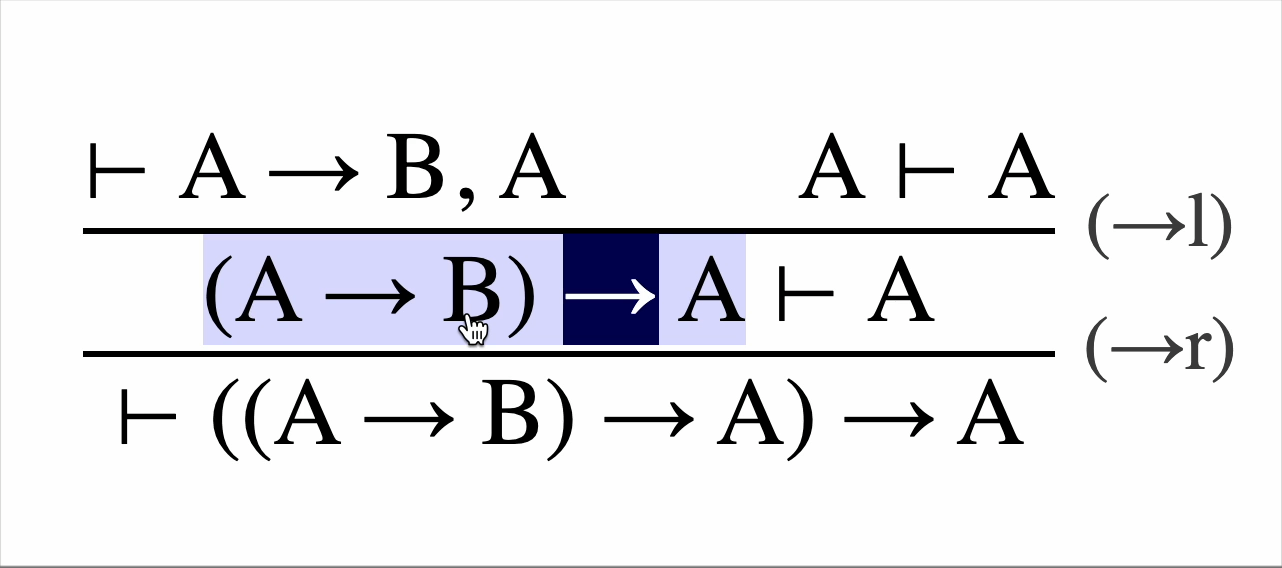
\includegraphics[width=\textwidth]{background/logitext-formula.png}
        \caption{Hovering over a formula}
    \end{subfigure}%
    \quad
    \begin{subfigure}{.48\textwidth}
        \centering
        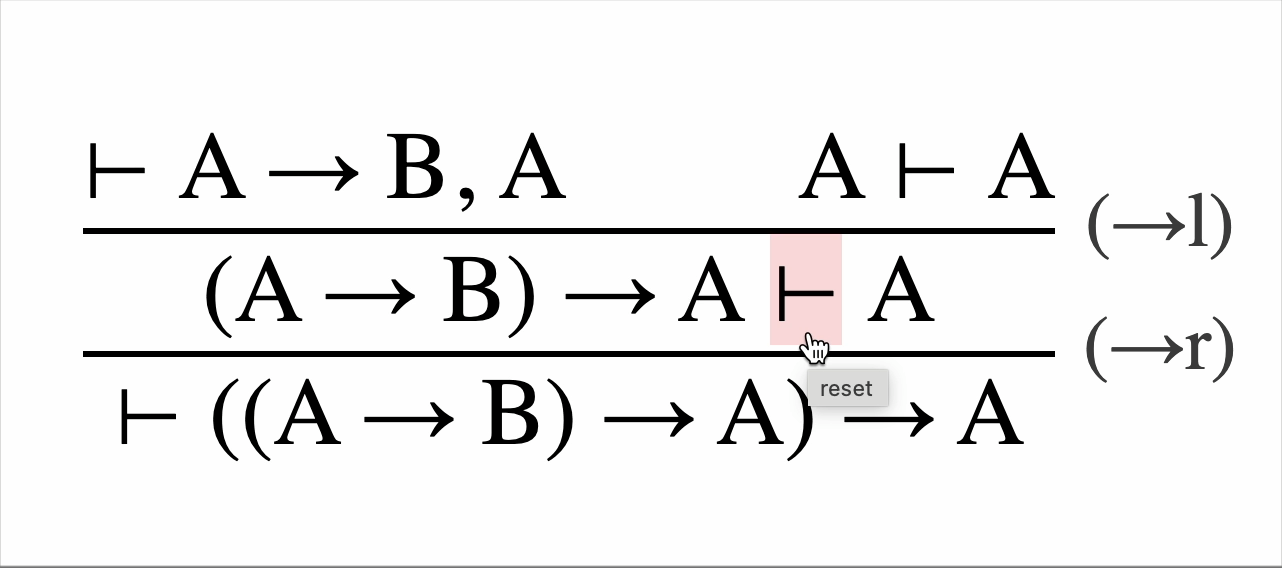
\includegraphics[width=\textwidth]{background/logitext-turnstile.png}
        \caption{Hovering over a turnstile}
    \end{subfigure}
    \caption{Lack of feedback when hovering over various parts of the derivation tree in Logitext}
    \label{fig:comparison:logitext}
\end{figure}

\paragraph{Helpful error messages}
When the user tries to apply an inference rule incorrectly, Logitext displays helpful and specific error messages, as seen in \Cref{fig:comparison:logitext-error}.

\begin{figure}[!htbp]
    \centering
    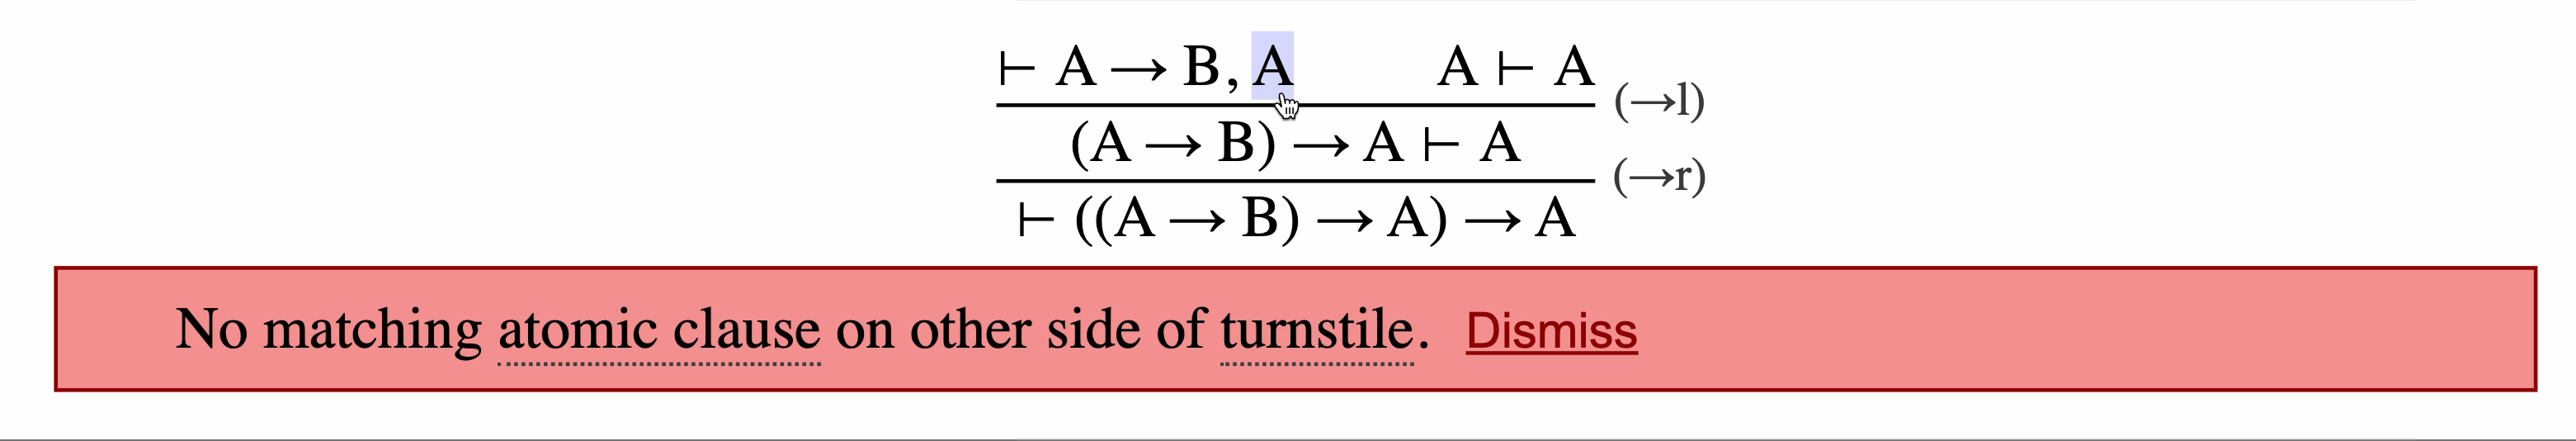
\includegraphics[width=\textwidth]{background/logitext-error.png}
    \caption{Helpful error messages in Logitext}
    \label{fig:comparison:logitext-error}
\end{figure}

\subsubsection{Flexibility}
Logitext only supports the system \textsc{lk}.

\subsection{Summary}
The application should retain the benefits and address the drawbacks of the proof assistants presented in this section. The desirable features of the application are as follows:
\begin{itemize}
    \item Users should be able to input statements in the application like writing statements by hand.
    \item The input syntax should either be already known by most users, or be easily accessible in the application.
    \item Users should be able to build derivations in the application like building derivations by hand.
    \item Users should be forced to think about which inference rule to apply and what the premises are. The application should not immediately rule out irrelevant inference rules.
    \item Users should be able to define both syntax and inference rules. The application should be as unopinionated about symbols as possible and designate as few special symbols as possible.
\end{itemize}